\subsection*{Partie I. Une formule d'Euler.}
\begin{enumerate}
 \item L'ensemble $\mathcal E(x)$ est fini de cardinal $\lfloor x\rfloor$. L'ensemble $\mathcal N(x)$ est infini car $\mathcal P(x)$ est fini (de cardinal $\pi(x)$) mais les exposants des facteurs premiers sont arbitraires. En revanche si on limite les exposants (entre $0$ et $m$) on obtient l'ensemble fini $\mathcal N_m(x)$ de cardinal $(m+1)^{\pi(x)}$.\newline
Pour $x$ fixé, tous les facteurs premiers des éléments de $\mathcal E(x)$ sont dans $\mathcal P(x)$. Notons $m$ le plus grand des exposants figurant dans ces décompositions. On a alors $\mathcal E(x)\subset\mathcal N_m(x)$. Comme $\mathcal N_m(x)$ est fini, il admet un plus grand élément $y$ on a bien alors $\mathcal N_m(x)\subset \mathcal E(y)$. Pour des $x$, $m$, $y$ vérifiant ces inclusions, on a $ Z_x \leq S_m(x) \leq Z_y$.

\item Quand on développe le produit proposé, on obtient une somme de $(m+1)^{\pi(x)}$ termes. Notons $q=\pi(x)$, chaque terme est de la forme
 $\frac{1}{\left(p_1^{m_1}p_2^{m_2}\cdots p_q^{m_q} \right)^\delta}$
avec  $(m_1,\cdots,m_q)\in\{0,\cdots,m\}^q$.\\ On obtient ainsi dans les dénominateurs tous les éléments de $\mathcal N_m(x)$ ce qui prouve la relation demandée. 
\item \begin{enumerate}
 \item L'encadrement demandé vient de l'inégalité des accroissements finis appliquée à la fonction $x\rightarrow x^{1-\delta}$ entre $j$ et $j+1$. Comme $\delta>1$, la dérivée $(1-\delta)x^{-\delta}$ est croissante (elle est aussi à valeurs négatives). On en déduit :
\begin{multline*}
 (1-\delta)(j)^{-\delta}\leq(j+1)^{1-\delta}-j^{1-\delta}\leq (1-\delta)(j+1)^{-\delta}\\ \Leftrightarrow
 \frac{\delta -1}{(j+1)^\delta}\leq \frac{1}{j^{\delta -1}} - \frac{1}{(j+1)^{\delta -1}}\leq 
\frac{\delta -1}{j^\delta}
\end{multline*}

\item On somme les inégalités précédentes; celle de gauche pour $j$ entre $1$ et $i-1$, puis celle de droite pour $j$ entre $1$ et $i$ :
\begin{multline*}
 \left.
\begin{aligned}
 \frac{\delta -1}{2^\delta}\leq& \frac{1}{1^{\delta -1}} - \frac{1}{2^{\delta -1}}\\
 \frac{\delta -1}{3^\delta}\leq& \frac{1}{2^{\delta -1}} - \frac{1}{3^{\delta -1}}\\
                              \vdots& \\
 \frac{\delta -1}{i^\delta}\leq& \frac{1}{(i-1)^{\delta -1}} - \frac{1}{i^{\delta -1}}
\end{aligned}
 \right\rbrace \Rightarrow
(\delta -1)(Z_i-1)\leq 1- \frac{1}{i^{\delta -1}}\\
\Rightarrow
Z_i \leq \frac{1}{\delta -1} +1 - \frac{1}{(\delta -1)i^{\delta -1}}
\end{multline*}
\begin{multline*}
 \left.
\begin{aligned}
  \frac{1}{1^{\delta -1}} - \frac{1}{2^{\delta -1}}\leq& \frac{\delta -1}{1^\delta}\\
 \frac{1}{2^{\delta -1}} - \frac{1}{3^{\delta -1}}\leq& \frac{\delta -1}{2^\delta}\\
                              \vdots& \\
  \frac{1}{i^{\delta -1}} - \frac{1}{(i+1)^{\delta -1}}\leq& \frac{\delta -1}{i^\delta}
\end{aligned}
 \right\rbrace \Rightarrow
 1- \frac{1}{(i+1)^{\delta -1}}\leq (\delta -1)Z_i\\
\Rightarrow
\frac{1}{\delta -1} - \frac{1}{(\delta -1)(i+1)^{\delta -1}}\leq Z_i
\end{multline*}

\item La suite $\left( Z_i \right)_{i\in\N^*}$ est clairement croissante par définition. La partie droite de l'encadrement précédent montre qu'elle est majorée par $\frac{1}{\delta -1}+1$. Elle est donc convergente et on note $\zeta(\delta)$ sa limite.\newline
On utilise encore l'encadrement mais cette fois avec le théorème de passage à la limite dans une inégalité, on obtient :
\begin{displaymath}
 \frac{1}{\delta -1} \leq \zeta(\delta) \leq \frac{1}{\delta -1} +1
\end{displaymath}
car $\delta$ étant $>1$ les termes en $\frac{1}{i^{\delta-1}}$ tendent vers $0$. 
\item La suite $\left(S_m(x) \right)_{m\in\N^*}$ est clairement croissante. D'après la première question, il existe un entier $i$ tel que $S_m(x)\leq Z_i\leq \zeta(\delta)$. La suite est donc majorée donc convergente et sa limite $S(x)$ vérifie $S(x)\leq\zeta(\delta)$.
\end{enumerate}
\item La suite est formée de sommes de termes d'une suite géométrique de raison $p^{-\delta}<1$
\begin{displaymath}
 \sum_{k=0}^{m}\frac{1}{p^{k\delta}}=\dfrac{1-p^{-(m+1)\delta}}{1-p^{-\delta}}\rightarrow \dfrac{1}{1-\frac{1}{p^\delta}}
\end{displaymath}
\item Pour tout entier $m$ et tout nombre premier $p$:
\begin{displaymath}
 \sum_{k=0}^{m}\frac{1}{p^{k\delta}}\leq \dfrac{1}{1-\frac{1}{p^\delta}}
\end{displaymath}
Considérons alors la suite  $\left(S_m(x)\right)_{m\in\N^*}$, d'après 1.
\begin{displaymath}
 S_m(x)=\prod_{p\in \mathcal P(x)}\left( \sum_{k=0}^{m}\frac{1}{p^{k\delta}}\right)
\end{displaymath}
La suite considérée est donc le produit des $\pi(x)$ suites convergentes $\left( \sum_{k=0}^{m}\frac{1}{p^{k\delta}}\right)_{m\in \N^*}$ pour $p$ décrivant $\mathcal P(x)$. Le produit d'une famille finie de suites convergentes est convergente et sa limite est le produit des limites. On en déduit que
\begin{displaymath}
 S(x)=\prod_{p\in \mathcal P(x)}\dfrac{1}{1-\frac{1}{p^\delta}}
\end{displaymath}
La question 3.d. montre que, pour $x$ fixé et $m$ assez grand 
\begin{displaymath}
 Z_x\leq S_m(x)\leq \prod_{p\in \mathcal P(x)}\dfrac{1}{1-\frac{1}{p^\delta}}\leq \zeta(\delta)
\end{displaymath}
Or $Z_x$ tend vers $\zeta(\delta)$ en $+\infty$. Le théorème d'encadrement entraîne alors la convergence du produit avec
\begin{displaymath}
  \lim_{x\rightarrow \infty }\prod_{p\in \mathcal P(x)}\frac{1}{1-\frac{1}{p^\delta}}=\zeta(\delta)
\end{displaymath}
\end{enumerate}

\subsection*{Partie II. Constante d'Euler.}
\begin{enumerate}
 \item \begin{enumerate}
 \item L'inégalité demandée résulte de l'inégalité des accroissements finis appliquée à la fonction $\ln$ entre $i$ et $i+1$ en tenant compte de la décroissance de la dérivée.  
\item Par définition de $u_n$ et d'après a.:
\begin{displaymath}
 u_{n+1}-u_n=\frac{1}{n+1}-\ln(n+1)+\ln n \leq 0
\end{displaymath}
ce qui prouve que $\left(u_n \right)_{n\in\N^*}$ est décroissante.
\item On somme les inégalités droites du a.
\begin{displaymath}
\left.  \begin{aligned}
  \ln 2 -& \ln 1 &\leq& \;\frac{1}{1}\\
  \ln 3 -& \ln 2 &\leq& \;\frac{1}{2}\\
         &         &\vdots &       \\
  \ln n -& \ln (n-1) &\leq& \;\frac{1}{n-1}\\
 \end{aligned}
\right\rbrace \Rightarrow
\ln n \leq 1+\frac{1}{2}+\cdots+\frac{1}{n-1} \Rightarrow
0\leq u_n - \frac{1}{n}
\end{displaymath}

\item La suite $\left(u_n \right)_{n\in\N^*}$ est décroissante d'après b et minorée par 0 (à valeurs positives) d'après c. Elle est donc convergente. On note $\gamma$ sa limite. On pose $v_n=u_n-\gamma$, la suite $\left(v_n \right)_{n\in\N^*}$ est décroissante et à valeurs positives.
\end{enumerate}

\item Notons $\varphi(x)$ l'expression dont on veut montrer qu'elle est positive. La fonction $\varphi$ est $\mathcal C^\infty$ dans $[0,1[$ et nulle en $0$. calculons la dérivée :
\begin{displaymath}
 \varphi'(x)=\underset{=0}{\underbrace{1-\frac{1}{1-x}+\frac{x}{1-x}}}+\frac{x^2}{2(1-x)^2}\geq 0
\end{displaymath}
La fonction $\varphi$ est donc croissante, nulle en $0$; elle est à valeurs positives.\newline
Calculons $\varphi(\frac{1}{n+1})$.
\begin{multline*}
 \varphi(\frac{1}{n+1})= \frac{1}{n+1} +\ln (1-\frac{1}{n+1})+\frac{1}{2(n+1)^2(1-\frac{1}{n+1})}\\
= \frac{1}{n+1} +\ln (1-\frac{1}{n+1})+\frac{1}{2(n+1)n}
\end{multline*}

\item Pour montrer que $\left(w_n \right)_{n\in\N^*}$ est croissante, formons $w_{n+1}-w_n$ avec 
\begin{displaymath}
 w_n = 1+\frac{1}{2}+\cdots+\frac{1}{n}-\ln n -\gamma -\frac{1}{2n}
\end{displaymath}
\begin{multline*}
 w_{n+1}-w_n = \frac{1}{n+1}-\ln(n+1)-\frac{1}{2(n+1)}+\ln n +\frac{1}{2n}\\
= \frac{1}{n+1} +\ln \frac{(n+1)-1}{n+1}+\left(\frac{1}{2n}-\frac{1}{2(n+1)} \right) \\
= \frac{1}{n+1}+\ln\left(1-\frac{1}{n+1}\right)+\frac{1}{2n(n+1)}\geq 0 
\end{multline*}
La suite $\left(w_n \right)_{n\in\N^*}$ est obtenue à partir de la suite $\left(v_n \right)_{n\in\N^*}$ qui tend vers $0$ en ajoutant un terme correctif $-\frac{1}{2n}$ qui converge vers $0$. Comme elle est croissante, cela entraîne qu'elle est à valeurs négatives ou nulles ce qui donne l'inégalité à droite de l'encadrement demandé
\begin{displaymath}
 0\leq Z_n-\ln n-\gamma\leq \frac{1}{2n}
\end{displaymath}
On avait déjà la positivité d'après 1.d.
\item Le raisonnement est très proche de celui des questions 2. et 3. Notons $\psi(x)$ l'expression dont on veut montrer qu'elle est positive. La fonction $\psi$ est $\mathcal C^\infty$ dans $[0,1[$ et nulle en $0$. Calculons la dérivée :
\begin{displaymath}
 \psi'(x)=1-\frac{1}{1-x}+\frac{x}{1+x}-\frac{x^2}{2(1+x)^2}
= -\frac{x^2}{1-x^2}-\frac{x^2}{2(1+x)^2} \leq 0
\end{displaymath}
On en déduit
\begin{multline*}
 \psi(\frac{1}{n+1})=\frac{1}{n+1} +\ln (1-\frac{1}{n+1})+\frac{1}{2(n+1)^2(1+\frac{1}{n+1})}\\
= \frac{1}{n+1} +\ln (1-\frac{1}{n+1})+\frac{1}{2(n+1)(n+2)}\leq 0
\end{multline*}
Formons $t_{n+1}-t_n$ avec 
\begin{displaymath}
 t_n = 1+\frac{1}{2}+\cdots+\frac{1}{n}-\ln n -\gamma -\frac{1}{2(n+1)}
\end{displaymath}
\begin{multline*}
 t_{n+1}-t_n = \frac{1}{n+1}-\ln(n+1)-\frac{1}{2(n+2)}+\ln n +\frac{1}{2(n+1)}\\
= \frac{1}{n+1} +\ln \frac{(n+1)-1}{n+1}+\left(\frac{1}{2(n+1)}-\frac{1}{2(n+2)} \right) \\
= \frac{1}{n+1}+\ln\left(1-\frac{1}{n+1}\right)+\frac{1}{2(n+1)(n+2)}\leq 0 
\end{multline*}
Comme la suite $\left(t_n \right)_{n\in\N^*}$ converge vers $0$ en décroissant, elle est à valeurs positives. Cela donne l'inégalité à droite de l'encadrement suivant, l'inégalité à gauche venant de la question 3.
\begin{displaymath}
 \frac{1}{2(n+1)}\leq Z_n - \ln n -\gamma \leq \frac{1}{2n}
\end{displaymath}
En divisant par $\frac{1}{2n}$, les suites de chaque côté tendent vers $1$ et on obtient par le théorème d'encadrement que
\begin{displaymath}
  Z_n - \ln n -\gamma \sim \frac{1}{2n}
\end{displaymath}

\end{enumerate}

\subsection*{Partie III. Valeur moyenne du nombre de diviseurs}
\begin{figure}[ht]
 \centering
 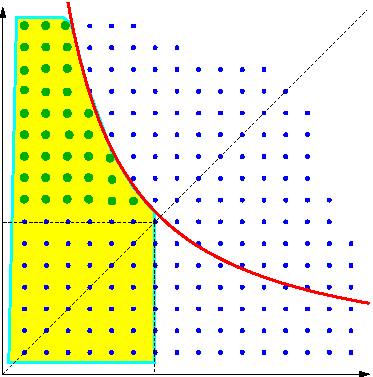
\includegraphics{Cthean_1.pdf}
 \caption{III.2. $\mathcal T = \mathcal C \cup \mathcal T_1$.}
 \label{fig:Cthean_1}
\end{figure}

\begin{enumerate}
 \item La définition de la relation de domination est : il existe $A>1$ et $M>0$ tel que $\frac{|f(x)-g(x)|}{|h(x)|}\leq M$ pour tous les $x\geq A$.
 
\item Les disques situés sur l'hyperbole de Dirichlet sont associés aux diviseurs de $x$, chaque coordonnée est un diviseur, le nombre $\tau(x)$ de diviseurs de $x$ est donc le nombre de disques sur l'hyperbole. Si $x$ et $y$ sont distincts, les hyperboles $\mathcal{H}_x$ et $\mathcal{H}_y$ sont disjointes. Pour les points du plan à coordonnées entières situés au dessous de $\mathcal{H}_x$, les hyperboles $\mathcal{H}_y$ avec $0<y\leq x$ forment une partition. On en déduit que la somme $D(x)$ des nombres de diviseurs des entiers plus petits que $x$ est le nombre total de disques au dessous de l'hyperbole.\newline
Notons $y$ l'ordonnée marquée par un point d'interrogation. On a $ym<x$ car le point est strictement au dessous de l'hyperbole et $(y+1)m>x$ d'ou $y<\frac{x}{m}<y+1$ donc
\begin{displaymath}
 y=\lfloor\frac{x}{m}\rfloor
\end{displaymath}
Notons $\mathcal D$ l'ensemble des points à coordonnées entières en dessous de l'hyperbole et $\mathcal C$ le carré indiqué sur la figure. Il est formé par les couples d'entiers $(m,k)$ tous les deux entre $1$ et $\lfloor\sqrt{x}\rfloor$. On a donc $\sharp \mathcal C = \lfloor\sqrt{x}\rfloor^2$.\newline
Notons $\mathcal T$ la zone délimitée sur la figure \ref{fig:Cthean_1}. Elle est formée par les couples d'entiers $(m,k)$ tels que $mk\leq x$ et $m<\sqrt{x}$. Chaque colonne de $\mathcal T$ d'abscisse $m$ est constituée par les $(m,k)$ avec $k$ entre $1$ et $\lfloor\frac{x}{m}\rfloor$ donc
\begin{displaymath}
 \sharp \mathcal T = \sum_{m\in \mathcal E(\sqrt{x})}\lfloor\frac{x}{m}\rfloor
\end{displaymath}
La partie $\mathcal T$ est l'union du carré $\mathcal C$ et de la partie au dessus notée $\mathcal T_1$ et représentée sur la figure par les plus gros disques. On peut définir une partie $\mathcal T_2$ symétrique de $\mathcal T_1$ par rapport à la bissectrice des axes. On a alors une union disjointe :
\begin{displaymath}
 \mathcal D = \mathcal T_1 \cup \mathcal C \cup \mathcal T_2
\end{displaymath}
Comme $\sharp \mathcal T_1=\sharp \mathcal T_2$ et $\sharp\mathcal T = \sharp \mathcal T_1 +\sharp \mathcal C$, on obtient :
\begin{displaymath}
 \sharp \mathcal D = 2\sharp \mathcal T - \sharp \mathcal C
\Rightarrow D(x) = 2\sum_{m\in \mathcal E(\sqrt{x})}\lfloor\frac{x}{m}\rfloor - \lfloor\sqrt{x}\rfloor^2
\end{displaymath}

\item Par définition de la partie entière et en sommant sur les $\lfloor\sqrt{x}\rfloor$ éléments de $\mathcal E(\sqrt{x})$:
\begin{align*}
  \frac{x}{m}-1 < \lfloor\frac{x}{m}\rfloor \leq \frac{x}{m} \\
xZ_{\sqrt{x}}-\lfloor\sqrt{x}\rfloor \leq \sum_{m\in\mathcal E(\sqrt{x})}\lfloor\frac{x}{m}\rfloor
\leq xZ_{\sqrt{x}}
\end{align*}
De $\lfloor\sqrt{x}\rfloor\leq \sqrt{x}$, on déduit l'encadrement demandé.

\item D'après les deux précédentes questions,
\begin{displaymath}
 2xZ_{\sqrt{x}}-2\lfloor\sqrt{x}\rfloor \leq D(x) +\lfloor\sqrt{x}\rfloor^2
\leq 2xZ_{\sqrt{x}}
\end{displaymath}
%%% \newcommand{\lfloor\sqrt{x}\rfloor}{\lfloor\sqrt{x}\rfloor}
Prouver le résultat revient à montrer que 
\begin{displaymath}
 \theta(x)=\sqrt{x}\left[\frac{D(x)}x-(\ln x+2\gamma-1)\right] 
\end{displaymath}
est borné au voisinage de $+\infty$.\newline
D'après la question 2., on a 
$$D(x)=2\sum_{m \in \mathcal{E}(\sqrt x)}\lfloor \frac xm\rfloor-\lfloor \sqrt x\rfloor^2$$
Donc par la question 3.:
\begin{displaymath}
2Z_{\sqrt{x}}-\frac{2\sqrt x}x-\frac{\lfloor\sqrt x\rfloor^2}x\ie \frac{D(x)}x\ie 2Z_{\sqrt{x}}-\frac{\lfloor\sqrt x\rfloor^2}x.  
\end{displaymath}
Or $Z_{\sqrt{x}}=Z_{\lfloor\sqrt{x}\rfloor}$, donc  par II 4., $Z_{\sqrt{x}}=\ln \lfloor\sqrt{x}\rfloor+\gamma+\frac{\varepsilon(\lfloor\sqrt{x}\rfloor)}{2\lfloor\sqrt{x}\rfloor}$ avec $\varepsilon\to_{+\infty} 1$.\\
D'une part, 
$$\theta(x)\ie \sqrt{x}
 \left[
  \ln\left(\frac{\lfloor\sqrt{x}\rfloor^2}x\right)
 +\frac{\varepsilon(\lfloor\sqrt{x}\rfloor)}{\lfloor\sqrt{x}\rfloor} 
 + 1-\frac{\lfloor\sqrt{x}\rfloor^2}x
 \right]$$
comme
\begin{itemize}
\item[$\ast$] $\lfloor\sqrt{x}\rfloor^2\ie x$ d'où $\sqrt{x}\ln\left(\frac{\lfloor\sqrt{x}\rfloor^2}x\right)\ie 0$.
\item[$\ast$] $\frac {\sqrt x}{\lfloor\sqrt{x}\rfloor}\varepsilon(\lfloor\sqrt{x}\rfloor)\to_{+\infty} 1$ donc $\frac {\sqrt x}{\lfloor\sqrt{x}\rfloor}\varepsilon(\lfloor\sqrt{x}\rfloor)$ est majoré au voisinage de $+\infty$.
\item[$\ast$] En minorant $\lfloor\sqrt{x}\rfloor$ par $\sqrt x-1$ on trouve que $\sqrt{x}\left( 1-\frac{\lfloor\sqrt{x}\rfloor^2}x\right) \ie 2$.   
\end{itemize}
On en déduit que la fonction $\theta$ est majorée au voisinage de $+\infty$.\\
D'autre part, 
\begin{displaymath}
\theta(x)\se \sqrt{x}\left[ 
     \ln\left( \frac{\lfloor\sqrt{x}\rfloor^2}x \right)
    + \frac{ \varepsilon(\lfloor\sqrt{x}\rfloor)}{\lfloor\sqrt{x}\rfloor} 
    + 1-\frac{\lfloor\sqrt{x}\rfloor^2}x-\frac{2\sqrt x}x 
 \right]  
\end{displaymath}
or
\begin{itemize}
\item[$\ast$] En minorant $\lfloor\sqrt{x}\rfloor$ par $\sqrt x-1$ on trouve que $\frac{\lfloor\sqrt{x}\rfloor^2}{x}\se 1-\frac{2}{\sqrt x}$, donc par croissance de $\ln$, puis en multipliant par $\sqrt x$ on obtient $\sqrt{x}\ln\left(\frac{\lfloor\sqrt{x}\rfloor^2}{x}\right)\se \sqrt{x}\ln\left(1-\frac{2}{\sqrt x}\right)$. Or $\sqrt{x}\ln\left(1-\frac{2}{\sqrt x}\right)\sim_{+\infty}-2$, et est donc minoré au voisinage de $+\infty$. Il en est donc de même pour $\sqrt{x}\ln\left(\frac{\lfloor\sqrt{x}\rfloor^2}{x}\right)$.
\item[$\ast$] $\lfloor\sqrt{x}\rfloor^2\ie x$ d'où $\sqrt x\left(1-\frac{\lfloor\sqrt{x}\rfloor^2}x\right)\se 0$. 
\item[$\ast$] $\frac {\sqrt x}{\lfloor\sqrt{x}\rfloor}\varepsilon(\lfloor\sqrt{x}\rfloor)\to_{+\infty} 1$, $\frac {\sqrt x}{\lfloor\sqrt{x}\rfloor}\varepsilon(\lfloor\sqrt{x}\rfloor)$ est donc minoré au voisinage de $+\infty$
\item[$\ast$] $-\sqrt x\, \left( \frac{2\sqrt x}x\right) = 2$.
\end{itemize}
On en déduit que la fonction $\theta$ est minorée au voisinage de $+\infty$.\\
La fonction $\theta$ est donc bornée au voisinage de $+\infty$.  
\end{enumerate}

\subsection*{Partie IV. Une inégalité de Chebychev}
\begin{enumerate}
 \item Par définition, $\theta(2)=\ln 2 < 2\ln 4 = \ln 16$.
 \item Lorsque $n$ est pair il n'est pas premier donc $\theta(n)=\theta(n-1)\leq (n-1)\ln 4 \leq n\ln 4 $.
 \item \begin{enumerate}
 \item Le développement de $(1+1)^{2m+1}$ est une somme de coefficients du binôme qui contient en particulier
\begin{displaymath}
 \binom{2m+1}{m} \text{ et }  \binom{2m+1}{m+1}=\binom{2m+1}{m}  
\end{displaymath}
On en déduit
\begin{displaymath}
 2\binom{2m+1}{m} \leq 2^{2m+1} \Rightarrow \binom{2m+1}{m}\leq 4^m
\end{displaymath}
\item Exprimons le coefficient du binôme avec des produits :
\begin{displaymath}
 \binom{2m+1}{m} = \frac{(2m+1)(2m)\cdots (m+1)}{m!}
\end{displaymath}
Les hypothèses sur le nombre premier $p$ montrent qu'il ne figure pas dans la décomposition de $m!$ mais qu'il apparait quelque part dans les facteurs du numérateur. Il divise donc ce coefficient du binôme.
\item Considérons $\theta(2m+1)-\theta(m+1)$. Il s'agit en fait d'une somme qui porte sur tous les nombres premiers $p$ de $\mathcal P(2m+1)\setminus \mathcal P(m+1)$ c'est à dire vérifiant les inégalités de la question b.
\begin{displaymath}
 \theta(2m+1)-\theta(m) = \sum_{p\in \mathcal P(2m+1)\setminus \mathcal P(m)}p
=\ln\left( \prod_{p\in \mathcal P(2m+1)\setminus \mathcal P(m)}p\right) 
\end{displaymath}
Comme tous les nombres premiers $p$ en jeu divisent le coefficient du binôme, leur produit le divise aussi. On en déduit
\begin{displaymath}
 \prod_{p\in \mathcal P(2m+1)\setminus \mathcal P(m)}p \leq \binom{2m+1}{m}
\Rightarrow
\theta(2m+1)-\theta(m) \leq \ln \binom{2m+1}{m}
\end{displaymath}
 
\end{enumerate}

\item Il s'agit ici d'achever la démonstration par récurrence ébauchée dans les premières questions. Définissons d'abord précisément la proposition. Pour $n$ naturel supérieur ou égal à 2:
\begin{displaymath}
 (\mathcal P_n)\hspace{1cm} \forall k\in\{2,\cdots,n\} : \theta(k)\leq k\ln 4
\end{displaymath}
La proposition $(\mathcal P_2)$ qui ne fait intervenir que $2$ a été montrée en question 1.\newline
On veut maintenant montrer que $(\mathcal P_{n-1})\Rightarrow(\mathcal P_{n})$ pour $n\geq 3$.
\begin{itemize}
 \item Le cas où $n$ est pair a été traité en 2.
\item Dans le cas où $n$ est impair et de la forme $2m+1$, on utilise la question 3. \`A cause du choix de la proposition à démontrer (récurrence forte), il suffit de majorer $\theta(n)$:
\begin{multline*}
 \theta(n) = \theta(2m+1)=\theta(m)+(\theta(2m+1)-\theta(m))
\leq m\ln 4 +\ln \binom{2m+1}{m}\\
\leq m\ln4 +\ln 4^m \leq 2m\ln 4 \leq n\ln 4
\end{multline*}
On a utilisé au passage la majoration trouvée de 3.a.
\end{itemize}

\end{enumerate}

